\documentclass[11pt]{article}
\usepackage[margin=1in]{geometry}
\usepackage{amsmath,amssymb,amsfonts,mathtools}
\usepackage{booktabs,multirow,array,tabularx}
\usepackage{graphicx}
\usepackage{tikz}
\usepackage{pgfplots}
\pgfplotsset{compat=1.17}
\title{Plot Sample 3}
\author{Dataset-expansion sample}
\date{}
\begin{document}
\maketitle
\section{Visualization}
The figure below is a TikZ/pgfplots drawing drawn from a source-backed image-to-LaTeX benchmark.

\begin{figure}[htbp]
\centering
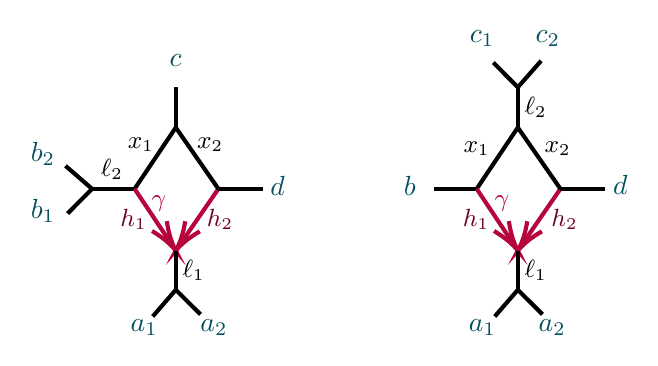
\begin{tikzpicture}
[x=0.75pt,y=0.75pt,yscale=-1,xscale=1]
\draw [line width=1.5] (52.05,101.79) -- (72.55,101.79) ;
\draw [line width=1.5] (72.55,101.79) -- (92.38,72.25) ;
\draw [color={rgb, 255:red, 182; green, 5; blue, 60 } ,draw opacity=1 ][line width=1.5] (72.55,101.79) -- (90.72,129.04) ;
\draw [shift={(92.38,131.54)}, rotate = 236.31] [color={rgb, 255:red, 182; green, 5; blue, 60 } ,draw opacity=1 ][line width=1.5] (14.21,-4.28) .. controls (9.04,-1.82) and (4.3,-0.39) .. (0,0) .. controls (4.3,0.39) and (9.04,1.82) .. (14.21,4.28) ;
\draw [color={rgb, 255:red, 182; green, 5; blue, 60 } ,draw opacity=1 ][line width=1.5] (112.9,101.79) -- (94.09,129.07) ;
\draw [shift={(92.38,131.54)}, rotate = 304.59] [color={rgb, 255:red, 182; green, 5; blue, 60 } ,draw opacity=1 ][line width=1.5] (14.21,-4.28) .. controls (9.04,-1.82) and (4.3,-0.39) .. (0,0) .. controls (4.3,0.39) and (9.04,1.82) .. (14.21,4.28) ;
\draw [line width=1.5] (112.9,101.79) -- (134.4,101.79) ;
\draw [line width=1.5] (92.38,131.54) -- (92.38,150.45) ;
\draw [line width=1.5] (92.38,72.25) -- (112.9,101.79) ;
\draw [line width=1.5] (92.38,52.84) -- (92.38,72.25) ;
\draw [line width=1.5] (104.28,162.26) -- (92.38,150.45) ;
\draw [line width=1.5] (81.28,163.26) -- (92.38,150.45) ;
\draw [line width=1.5] (216.85,101.79) -- (237.35,101.79) ;
\draw [color={rgb, 255:red, 0; green, 0; blue, 0 } ,draw opacity=1 ][line width=1.5] (237.35,101.79) -- (257.18,72.25) ;
\draw [color={rgb, 255:red, 182; green, 5; blue, 60 } ,draw opacity=1 ][line width=1.5] (237.35,101.79) -- (255.52,129.04) ;
\draw [shift={(257.18,131.54)}, rotate = 236.31] [color={rgb, 255:red, 182; green, 5; blue, 60 } ,draw opacity=1 ][line width=1.5] (14.21,-4.28) .. controls (9.04,-1.82) and (4.3,-0.39) .. (0,0) .. controls (4.3,0.39) and (9.04,1.82) .. (14.21,4.28) ;
\draw [color={rgb, 255:red, 182; green, 5; blue, 60 } ,draw opacity=1 ][line width=1.5] (277.7,101.79) -- (258.88,129.07) ;
\draw [shift={(257.18,131.54)}, rotate = 304.59] [color={rgb, 255:red, 182; green, 5; blue, 60 } ,draw opacity=1 ][line width=1.5] (14.21,-4.28) .. controls (9.04,-1.82) and (4.3,-0.39) .. (0,0) .. controls (4.3,0.39) and (9.04,1.82) .. (14.21,4.28) ;
\draw [color={rgb, 255:red, 0; green, 0; blue, 0 } ,draw opacity=1 ][line width=1.5] (277.7,101.79) -- (299.2,101.79) ;
\draw [color={rgb, 255:red, 0; green, 0; blue, 0 } ,draw opacity=1 ][line width=1.5] (257.18,131.54) -- (257.18,150.45) ;
\draw [color={rgb, 255:red, 0; green, 0; blue, 0 } ,draw opacity=1 ][line width=1.5] (257.18,72.25) -- (277.7,101.79) ;
\draw [color={rgb, 255:red, 0; green, 0; blue, 0 } ,draw opacity=1 ][line width=1.5] (257.18,52.84) -- (257.18,72.25) ;
\draw [line width=1.5] (245.37,40.94) -- (257.18,52.84) ;
\draw [line width=1.5] (268.38,40.11) -- (257.18,52.84) ;
\draw [line width=1.5] (269.08,162.26) -- (257.18,150.45) ;
\draw [line width=1.5] (246.08,163.26) -- (257.18,150.45) ;
\draw [line width=1.5] (40.24,113.69) -- (52.05,101.79) ;
\draw [line width=1.5] (39.24,90.69) -- (52.05,101.79) ;
\draw (301.86,94.01) node [anchor=north west][inner sep=0.75pt] [font=\normalsize,color={rgb, 255:red, 6; green, 79; blue, 97 } ,opacity=1 ] {$d$};
\draw (201.04,94.61) node [anchor=north west][inner sep=0.75pt] [font=\normalsize,color={rgb, 255:red, 6; green, 79; blue, 97 } ,opacity=1 ] {$b$};
\draw (244.74,104.01) node [anchor=north west][inner sep=0.75pt] [font=\small,color={rgb, 255:red, 182; green, 5; blue, 60 } ,opacity=1 ] {$\gamma $};
\draw (55.05,86.24) node [anchor=north west][inner sep=0.75pt] [font=\small,color={rgb, 255:red, 0; green, 0; blue, 0 } ,opacity=1 ] {$\ell _{2}$};
\draw (229.79,77.79) node [anchor=north west][inner sep=0.75pt] [font=\small] {$x_{1}$};
\draw (268.79,77.79) node [anchor=north west][inner sep=0.75pt] [font=\small] {$x_{2}$};
\draw (232.83,24.4) node [anchor=north west][inner sep=0.75pt] [font=\normalsize,color={rgb, 255:red, 6; green, 79; blue, 97 } ,opacity=1 ] {$c_{1}$};
\draw (264.5,24.4) node [anchor=north west][inner sep=0.75pt] [font=\normalsize,color={rgb, 255:red, 6; green, 79; blue, 97 } ,opacity=1 ] {$c_{2}$};
\draw (136.63,94.31) node [anchor=north west][inner sep=0.75pt] [font=\normalsize,color={rgb, 255:red, 6; green, 79; blue, 97 } ,opacity=1 ] {$d$};
\draw (69.38,163.46) node [anchor=north west][inner sep=0.75pt] [font=\normalsize,color={rgb, 255:red, 6; green, 79; blue, 97 } ,opacity=1 ] {$a_{1}$};
\draw (88.18,35.6) node [anchor=north west][inner sep=0.75pt] [font=\normalsize,color={rgb, 255:red, 6; green, 79; blue, 97 } ,opacity=1 ] {$c$};
\draw (79.5,104.01) node [anchor=north west][inner sep=0.75pt] [font=\small,color={rgb, 255:red, 182; green, 5; blue, 60 } ,opacity=1 ] {$\gamma $};
\draw (64.45,110.51) node [anchor=north west][inner sep=0.75pt] [font=\small,color={rgb, 255:red, 108; green, 4; blue, 35 } ,opacity=1 ] {$h_{1}$};
\draw (94.38,134.94) node [anchor=north west][inner sep=0.75pt] [font=\small,color={rgb, 255:red, 0; green, 0; blue, 0 } ,opacity=1 ] {$\ell _{1}$};
\draw (68.05,75.79) node [anchor=north west][inner sep=0.75pt] [font=\small] {$x_{1}$};
\draw (102.98,163.46) node [anchor=north west][inner sep=0.75pt] [font=\normalsize,color={rgb, 255:red, 6; green, 79; blue, 97 } ,opacity=1 ] {$a_{2}$};
\draw (101.38,75.79) node [anchor=north west][inner sep=0.75pt] [font=\small] {$x_{2}$};
\draw (106.05,110.51) node [anchor=north west][inner sep=0.75pt] [font=\small,color={rgb, 255:red, 108; green, 4; blue, 35 } ,opacity=1 ] {$h_{2}$};
\draw (232.38,163.46) node [anchor=north west][inner sep=0.75pt] [font=\normalsize,color={rgb, 255:red, 6; green, 79; blue, 97 } ,opacity=1 ] {$a_{1}$};
\draw (265.98,163.46) node [anchor=north west][inner sep=0.75pt] [font=\normalsize,color={rgb, 255:red, 6; green, 79; blue, 97 } ,opacity=1 ] {$a_{2}$};
\draw (21.29,78) node [anchor=north west][inner sep=0.75pt] [font=\normalsize,color={rgb, 255:red, 6; green, 79; blue, 97 } ,opacity=1 ] {$b_{2}$};
\draw (21.29,105.61) node [anchor=north west][inner sep=0.75pt] [font=\normalsize,color={rgb, 255:red, 6; green, 79; blue, 97 } ,opacity=1 ] {$b_{1}$};
\draw (229.45,110.51) node [anchor=north west][inner sep=0.75pt] [font=\small,color={rgb, 255:red, 108; green, 4; blue, 35 } ,opacity=1 ] {$h_{1}$};
\draw (272.05,110.51) node [anchor=north west][inner sep=0.75pt] [font=\small,color={rgb, 255:red, 108; green, 4; blue, 35 } ,opacity=1 ] {$h_{2}$};
\draw (259.18,134.94) node [anchor=north west][inner sep=0.75pt] [font=\small,color={rgb, 255:red, 0; green, 0; blue, 0 } ,opacity=1 ] {$\ell _{1}$};
\draw (259.18,56.24) node [anchor=north west][inner sep=0.75pt] [font=\small,color={rgb, 255:red, 0; green, 0; blue, 0 } ,opacity=1 ] {$\ell _{2}$};
\end{tikzpicture}
\caption{Source-backed plot.}
\end{figure}

\end{document}
